%% Environmetrics (Wiley) submission — guideline-compliant layout
%% 12pt, double spaced, <=26 lines/page, >=1in margins, numbered pages
\documentclass[12pt]{article}
\usepackage[utf8]{inputenc}
\usepackage[T1]{fontenc}
\usepackage{times}
\usepackage[a4paper,margin=1in,textheight=8.7in]{geometry}  % caps the page at 26 double-spaced 12pt lines
\usepackage{setspace}
\usepackage{amsmath,amssymb}
\usepackage{graphicx}
\usepackage{booktabs}
\usepackage{siunitx}
\usepackage[round,authoryear]{natbib}
\usepackage{url}
\usepackage{lineno}
\bibliographystyle{apalike}
\newcommand{\pmten}{PM$_{10}$}
\newcommand{\pmtf}{PM$_{2.5}$}
\newcommand{\ugm}{\si{\micro\gram\per\cubic\metre}}
\begin{document}
\doublespacing
\title{\bf A dependence-pathway audit for spatial transfer: error rates of the
design and of its inference unit}
\author{}
\date{}
\maketitle
\thispagestyle{empty}
\begin{center}
\emph{Running title}: Error rates of a spatial-transfer audit and its inference unit
\end{center}
\begin{abstract}
We propose a dependence-pathway audit for the claim that a model fitted at monitored locations transfers to an unmonitored one. The audit removes the pathways connecting a held-out target to its training data --- spatial proximity, temporal co-location and shared grid support --- in turn, each control set from the measured dependence structure. On CAMS \pmten{} residual correction across 19 stations, three conventions flip the verdict. Because observed data cannot separate a design that suppresses a false claim from one that destroys a real signal, we measure the audit in a 32-scenario experiment with signal and pathways set by construction. Across 25-, 50- and 100-km buffers it holds false-positive verdicts near 2--3\%, rising to 11--13\% where a component common to the network in time makes the station-level sign test anti-conservative. A validation design also chooses the unit its verdict is counted over. Coarsening to grid cells does not repair that corner: an arbitrary grouping of the same size matches it. Cutting the units along time does repair it, at a smaller cost in detection. The unit should be cut along the dependence that threatens the test, not the one that is easiest to see.
\end{abstract}
\par\medskip\noindent\textbf{Keywords:} spatial cross-validation; spatial transferability; modifiable areal unit problem; validation design; geospatial machine learning
\clearpage
\section{Introduction}

This paper proposes a dependence-pathway audit for claims that a model fitted at monitored locations transfers to a location where no local observations exist, and measures how often that audit decides wrongly. The audit does not fix a block geometry in advance. It names the pathways through which a nominally held-out target can still be informed by its training data --- spatial proximity to surviving sources, co-location in time, shared mechanistic-grid support, and coordinates acting as station identifiers --- removes them in turn, and sets each control from the dependence structure measured in the data rather than from convention. Because a design that merely suppresses claims cannot be told from one that detects correctly on observed data, we then put the audit in an environment where the answer is known by construction and report its false-positive and detection rates, and those of the inference unit it counts over.

The reason a design is needed at all is that a spatial holdout is usually described as a degree of strictness: a random split is lenient, a blocked or buffered split is strict. It is better described as a choice of estimand. What a held-out location can be asked to establish depends on which information about it survives in the training set, and for spatially structured data a nominally held-out sample need not be informationally independent of what remains. Nearby monitoring sites may observe the same field; source and target sites may be observed at the same times; gridded mechanistic predictors may be identical at multiple stations; and coordinates or other spatial proxies may encode station identity. These problems are well established for random cross-validation and environmental mapping, motivating spatial blocking, leave-location-and-time-out designs, distance matching, explicit limits on a model's area of applicability, and tiered validation schemes that separate interpolation from geographic transfer \citep{roberts2017,valavi2019blockcv,meyer2018llto,mila2022nndm,linnenbrink2024knndm,meyer2021aoa,jiang2026tiered,pohjankukka2017skcv}. The gap between the two kinds of estimate is not marginal. Reproducing the standard mapping workflow on 11.8 million inventoried trees, \citet{ploton2020} obtained a nonspatial validation indicating that the model explained more than half the variation in forest biomass, and a spatial validation of the same model indicating quasi-null predictive power; in roof detection from satellite imagery the corresponding inflation reaches 17 percentage points, with cross-validated overall accuracies exceeding 99\% \citep{abriha2023}, and comparable effects are reported for seafloor nodule mapping \citep{gazis2021} and species-abundance models \citep{mushagalusa2024}. The general name for the mechanism is leakage, and its prevalence across machine-learning-based science is now itself an object of study \citep{kapoor2023leakage,kapoor2024reforms}. The more specific question considered here is whether a model fitted to residuals at monitored locations genuinely \emph{transfers} to a location at which no local observations are available. That target is not hypothetical. Ambient particulate matter remains among the leading environmental contributors to global mortality \citep{cohen2017}, regulatory networks are sparse relative to populated area, and even the aggregated open archives that pool them carry substantial gaps at most sites \citep{tan2022openaq,rosales2025}. Land-use regression and learned corrections are both used to issue values where no monitor stands \citep{zhang2018lur,wang2025lur}, so what a station holdout does and does not license applies to them directly.

The consequence is that a validation design defines an estimand, and the designs differ in which one they target: withholding one station while retaining nearby and simultaneous sources asks about interpolation within a monitored network; adding a spatial buffer asks about geographic separation; removing temporally adjacent sources asks whether skill persists when the same episode cannot be looked up elsewhere; excluding sources that share a mechanistic grid cell asks whether the correction depends on shared covariate support. None is universally correct, because the relevant design depends on what information would exist at deployment. Direct transfer designs built on mutually disjoint geographic units are one strong answer where such units exist \citep{patane2025}, but many monitoring networks require internal stress tests of the pathways that remain. The distance-buffered form used here has a precedent: \citet{pohjankukka2017skcv} withhold a dead zone of chosen radius around each test point and report ordinary cross-validation up to 40\% more optimistic than the buffered estimate. What that construction fixes is the optimism of a performance estimate; what it leaves open, and what is asked here, is how the radius should be chosen and how often the resulting design decides wrongly in either direction. A useful audit must do two things at once: suppress false claims of transfer caused by residual dependence, and retain enough power to detect transferable structure when it exists.

Residual correction differs from generic environmental mapping in a consequential way. The learner does not predict the quantity from scratch; it learns the discrepancy between a spatially complete mechanistic field and observations and adds it back. This is the standard form of operational air-quality post-processing \citep{djalalova2010,djalalova2015,huang2017,zhang2021ens,ye2022,skipper2024,miyazaki2025}, inside the wider statistical-postprocessing tradition from which its evaluation conventions are inherited \citep{vannitsem2021,rasp2018,schulz2022}. It also creates multiple dependence pathways at once: a withheld target may remain close to source monitors, share their timestamps, and share the same coarse mechanistic grid cell, so even a coordinate-free residual model can retain location information through the mechanistic predictor itself.

Prior work has shown that spatial proxies can support interpolation while failing under extrapolation and that the validation design can strongly determine apparent generalization \citep{mila2024proxies,wadoux2021}. Recent studies reinforce the distinction between fit within observed spatial support and transfer beyond it: coordinate-based spatial terms can improve residual spatial structure without guaranteeing spatial generalization, and local environmental support can govern extrapolative performance \citep{pompili2026,portes2026}. A parallel line measures the dissimilarity between the sample and the prediction locations in feature space rather than in geographic space, and makes the validation design follow it: \citet{wang2023spatialplus} split folds by clustering locations, covariates and target together, \citet{wang2025adversarial} quantify the sample-to-prediction dissimilarity with a binary classifier and report that which cross-validation design is least biased depends on how large that dissimilarity is, and \citet{wang2025dissimilarity} let the fold construction adapt to it. \citet{linnenbrink2026beyond} gather these into a prediction-domain adaptive category and argue that independence between training and evaluation data is not the goal, because enforcing it creates an extrapolation the deployed model will not face. Less attention has been paid to the joint contribution of temporal co-location, shared mechanistic-grid support, and data-selection rules in cross-location residual transfer. The same question has been put from the model-based side. \citet{adin2024lgocv} show that leave-one-out cross-validation is not generally suitable for models carrying structured random effects, because correlation between the training and the test set enters the estimated prediction error, and compare it against automatic leave-group-out construction in latent Gaussian models; \citet{lobo2020bayescv} make the choice of validation locations itself an object of inference for geostatistical models, averaging predictive discrepancy over partitions rather than conditioning on one. Both act on the estimate; the controls examined here act on the information pathways that produce it. A related strand makes the diagnostic itself spatially explicit rather than the fold construction: \citet{brenning2023diagnostics} reports model-agnostic performance and variable importance as functions of prediction distance, and \citet{wiedemann2025geot} assemble spatially explicit error measures into an evaluation framework for spatio-temporal predictions. These describe how error varies over space; the question here is whether a transfer claim should be declared at all, which converts an error surface into a decision and so calls for false-positive and detection rates instead. Two recent studies establish the value of evaluating a validation design against a known answer rather than against another validation design. \citet{stock2025blocks} generates 1{,}426 synthetic data sets mimicking a satellite chlorophyll-\emph{a} mapping problem, in which prediction error is known everywhere, and asks how block size, block shape, fold count and fold assignment change the estimated accuracy; block size dominates, and no strategy returns an unbiased estimate. \citet{koldasbayeva2025stcv} hold out external out-of-time test sets for two real presence--absence data sets and show that random cross-validation overstates AUC by as much as $0.16$, while blocking at the \emph{measured} spatial autocorrelation range removes most of that bias. Both ask what a cross-validation design estimates, and so does the most recent synthesis of the field: \citet{linnenbrink2026beyond} reproduce and extend a simulation comparison of evaluation methods, and the quantity compared is the estimated error against the true error under four sampling designs. None of them asks the question that follows once the design is used to \emph{decide} something: given a design, how often is a transfer claim declared when none is present, and how often is a real one missed. A multi-author review of the field names the gap from the other side, reporting that the absence of systematic benchmarking continues to constrain comparison between the methods that incorporate spatial information into machine learning \citep{nowosad2026navigating}. That question needs the signal itself to be switched on and off by construction, which is the experiment reported here. \citet{mahoney2023assessing} come closest on the first count, comparing five spatial cross-validation methods by simulation, but the quantity they compare is again the accuracy estimate rather than a decision. On the second count, \citet{brenning2026aligning} argue concurrently and independently that validation should be aligned with deployment, and do it by re-weighting the existing validation sample so that its task distribution matches a target domain, which addresses preferential and clustered sampling. The alignment pursued here is the complementary one: rather than re-weighting the sample, we remove the information pathways that would be absent at deployment, and we measure how often the resulting design decides wrongly.

We develop such an audit and evaluate it in two complementary settings, one of which has a known answer. The demonstration uses CAMS \pmten{} residual correction across a dense 19-station monitoring network in the Abu Dhabi Emirate. The empirical audit progressively separates source and target stations in space, time and mechanistic-grid support, crosses these controls with a coordinate-free ablation, and sets key validation parameters from the measured data structure rather than from convention. Second, because a real network cannot reveal whether the underlying transferable signal is truly absent or merely difficult to detect, we construct a 32-scenario stochastic experiment in which the presence of genuine transfer, spatial dependence, temporal dependence, shared-grid dependence and network geometry are known by design. The central question is therefore not whether the strictest holdout produces the lowest apparent skill. It is what evidence is required before an apparent gain can be interpreted as spatial transfer, and what power is lost as dependence pathways are progressively blocked.

\section{Materials and Methods}

\subsection{Residual-transfer problem and target estimand}

Let $m_i(t)$ denote the mechanistic prediction at station $i$ and time $t$, $y_i(t)$ the observation, and
\begin{equation}
 r_i(t)=y_i(t)-m_i(t)
\end{equation}
the mechanistic-model residual. A residual corrector $f(\cdot)$ is fitted using observations from source stations and predicts $\widehat r_i(t)$ for a held-out target station. The corrected mechanistic prediction is
\begin{equation}
 \widehat y_i(t)=m_i(t)+\widehat r_i(t).
\end{equation}
We quantify target-station improvement with
\begin{equation}
 \Delta_i=\log\left(\frac{\mathrm{MAE}_{\mathrm{raw},i}}{\mathrm{MAE}_{\mathrm{transfer},i}}\right),
\end{equation}
where positive $\Delta_i$ indicates that the transferred correction improves upon the uncorrected mechanistic field. This log error ratio is the primary transfer estimand in both the empirical audit and the stochastic experiment.

We distinguish four increasingly separated questions. A target-station holdout asks whether a model trained on the remaining network improves a held-out location. A spatially buffered holdout additionally asks whether that improvement survives the removal of nearby source stations. A spatial--temporal holdout asks whether it survives when source observations from the held-out target period and a guard interval are excluded. Finally, a shared-grid control removes source stations assigned to the same mechanistic-model grid cell as the target. These designs are diagnostic rungs rather than a ranking of universally superior validation procedures: each corresponds to a different information set that may or may not match the intended deployment.

\subsection{Environmental demonstration: observations and CAMS}

The primary empirical analysis uses the 19-station Abu Dhabi Emirate regulatory \pmten{} network assembled from the OpenAQ archive \citep{rosales2025} for 2022--2023. Hourly observations were screened for sentinel and negative values and aggregated to the three-hourly CAMS time grid. The matched record contains 20,818 station--time observations before the final flat-line quality-control variants used in the audit. The network is spatially dense, with a median nearest-neighbour distance of 6.5~km, and the cold-start audit uses each station's available matched record. This density is useful for diagnosing interpolation but also makes ordinary leave-one-station-out validation particularly vulnerable to residual spatial dependence.

The mechanistic field is the Copernicus Atmosphere Monitoring Service global reanalysis EAC4, providing three-hourly surface \pmten{} at $0.75^{\circ}$ resolution \citep{inness2019,flemming2015}. The nearest CAMS grid cell was assigned to each station. Because the grid is much coarser than the monitoring network, multiple stations share an identical CAMS predictor series. Under the empirical $0.75^{\circ}$ assignment, the 19 stations occupy nine CAMS cells; 15 of the 171 station pairs share a cell, involving 16 of the 19 stations, at separations up to approximately 46~km. This is not merely a representativeness issue: identical gridded predictor series constitute a direct information-sharing pathway in a residual-transfer model.

The question was raised by a forecasting benchmark, which asked whether a learned corrector beats the mechanistic field at a station carrying no local observations. That benchmark is not reported here and is not a co-equal research question: reproducible multi-model air-pollution benchmarks already exist \citep{chisilev2026}, and what is at issue in this article is the validity of a cold-start transfer claim rather than the ranking of forecasting architectures. Its code and outputs remain in the public repository.

\subsection{Multi-dependence validation ladder}

The empirical residual learner is a deterministic histogram gradient-boosting regressor \citep{friedman2001} with early stopping disabled and fixed random state, as implemented in \texttt{scikit-learn} \citep{pedregosa2011}. The coordinate-bearing feature set includes the CAMS value, cyclic hour and day-of-year terms, latitude and longitude. The coordinate-free specification removes latitude and longitude while retaining the mechanistic and temporal covariates. Because CAMS is sampled on a coarse grid, the coordinate-free specification should not be interpreted as location-free; the separate grid-cell control is required to diagnose that pathway.

The first rung is leave-one-station-out transfer. For each target, the model is fitted to all other stations and evaluated at the target. The second rung applies a distance buffer, removing all source stations within radius $R\in\{0,25,50,100\}$~km. Source counts are reported at every radius so that a loss of apparent skill can be distinguished from simple training-data starvation.

The third rung controls temporal co-location. Source and target stations in a monitoring network are often observed during the same episodes; with a date encoding, a nonlinear learner can use surviving sources to reconstruct the network-wide residual state at the target timestamp. Each target's record is therefore divided into six contiguous temporal blocks. When a block is evaluated, source observations within that block and within a guard interval on either side are removed from training. The final rung excludes every source station sharing the target's CAMS cell in addition to the spatial and temporal controls.

\subsection{Data-adaptive audit parameters}

Three audit parameters were set from the observed data structure rather than fixed solely by convention. First, the temporal guard was derived from the lag autocorrelation of the observation-minus-CAMS residual. The median station-level residual autocorrelation was $+0.19$ at three days and reached $+0.08$ only at ten days (Figure~\ref{fig:guard}a). The primary empirical audit therefore uses a ten-day guard, with three days retained as a sensitivity analysis. A guard interval placed on either side of a withheld block is the cross-location analogue of $hv$-block cross-validation for dependent series, in which adjacent observations are discarded so that the training and evaluation sets are approximately independent \citep{racine2000}. Whether such removal is required at all has been contested for purely autoregressive forecasting, where a model whose own residuals are serially uncorrelated can be evaluated on randomly partitioned folds without bias \citep{bergmeir2012,cerqueira2020}. That argument does not reach the present case: the observations removed by the guard belong to \emph{other} stations, so they do not encode the target's own past but the network-wide state of the episode the target is being asked to predict. The wider guard reduces the median training sample from 11,068 to 9,789 rows per fold, a loss of 11.6\%.

Second, temporal blocks are defined by quantiles of each target station's own timestamps rather than by equal calendar intervals. The observational record contains months with little or no data. Calendar-equal splitting therefore generated nearly empty folds, including folds with only 9, 4 and 7 observations at one station, and a median largest-to-smallest fold ratio of 124. Equal-count blocks instead contain approximately 170--190 observations per fold and reduce that imbalance ratio to 1.01 (Supplementary Information, \emph{Three conventions inside the audit}).

Third, the flat-line quality-control rule was treated as an evaluation-set construction choice rather than a neutral preprocessing constant. The primary rule removes runs of six or more identical consecutive observations, eliminating 1.2\% of the record. A more aggressive threshold of three repeated values removes 9.9\%. Because the observations are integer-valued and short ties are common, the removed sample is not random: under the aggressive threshold its median concentration is 60~\ugm{} versus approximately 74--75~\ugm{} for the network, and high-concentration observations are depleted. Both thresholds are therefore propagated through the same audit pipeline.

\subsection{Statistical inference and diagnostic controls}

The empirical inference unit is the held-out station, with CAMS grid cells also examined as a coarser clustering unit. For each target, $\Delta_i$ is computed from raw and transferred MAE. Uncertainty is assessed by station and grid-cell resampling with 2,000 bootstrap replicates \citep{efron1979}; resampling whole grid cells rather than individual stations is a block bootstrap taken over the dependent unit \citep{kunsch1989,politis1994}. Verdict rates in the stochastic experiment are reported with Wilson score intervals \citep{wilson1927}. Directional consistency is evaluated with exact sign tests and magnitude with Wilcoxon signed-rank tests \citep{wilcoxon1945}; false-discovery-rate correction is applied within pre-declared families using Benjamini--Hochberg adjustment \citep{benjamini1995}. Every paired contrast is reported with a paired effect size as well as a test: Cohen's $d_z$ with a bootstrap percentile interval over stations, and the matched-pairs rank-biserial correlation that belongs with the Wilcoxon signed-rank statistic. Coordinate-bearing and coordinate-free specifications are compared directly with the paired difference $\Delta_{\mathrm{coordfree}}-\Delta_{\mathrm{full}}$ rather than by comparing two separate significance decisions, following the general warning that a difference between ``significant'' and ``not significant'' is not itself evidence of a significant difference \citep{gelman2006}. The same caution governs aggregation across folds: training sets that overlap make fold-level statistics dependent, so tests treating folds as independent replicates understate their own variance \citep{dietterich1998,nadeau2003}. Verdicts in the stochastic experiment are therefore formed once per realization and aggregated across independent realizations, never across the folds within one.

The area-of-applicability and nearest-neighbour-distance diagnostics reported for both the observed and the simulated networks follow \citet{meyer2021aoa} and \citet{mila2024proxies} and are implemented in the \texttt{CAST} package \citep{meyer2024cast}; because the simulation runs in Python, the unweighted variants are reimplemented here rather than called from that package, and the reimplementation ships with the code. The question the area of applicability formalises --- whether a prediction point lies inside the region its training data can support --- is older than its spatial statement. Regulatory toxicology has required an explicit applicability domain for structure--activity models for the same reason, and reaches it through the same distance- and reliability-based constructions \citep{toplak2014,jang2025qsar}; applying that test to published acute-toxicity models shows how narrow the supported region can turn out to be once it is measured rather than assumed \citep{fisher2025ad}. Open-set recognition states the problem as detection instead, flagging inputs whose class was never in the training set rather than assuming a closed set holds \citep{kang2026openset}. The spatial case adds only that the coordinate deciding membership is geographic. Three additional diagnostics test the audit rather than the predictive model. A coordinate-permutation placebo scrambles station coordinates while keeping all other inputs fixed. A grid-origin sensitivity analysis shifts the nominal CAMS grid assignment over seven offsets. Source-set stability is evaluated by resampling source stations rather than random seeds, because the reported gradient-boosting estimator is deterministic. Finally, deployment geometry is compared with validation geometry by simulating locations within the network bounding box and measuring distance to the nearest monitor.

\subsection{Ground-truth stochastic experiment}

The empirical network cannot identify whether a strict audit removes false apparent transfer or suppresses a real but weak transferable signal. We therefore constructed a stochastic experiment with known ground truth. Explicit representation of spatial and temporal dependence is standard in multi-site stochastic environmental modelling \citep{chida2025}; here that structure is used as a controlled falsification environment for validation rather than as a forecasting model. For station $i$ and time $t$, the residual is generated by Equation~\eqref{eq:simulation},
\begin{equation}
 r_i(t)=\beta F_i(t)+S_i+T(t)+G_{c(i)}(t)+\epsilon_i(t),
 \label{eq:simulation}
\end{equation}
where $F_i(t)$ is a structurally transferable function of the mechanistic field and seasonality, $S_i$ is a spatially correlated station component drawn once per realization from a zero-mean Gaussian field with exponential covariance $\exp(-d_{ij}/\rho)$ at range $\rho=70$~km and standardized to unit variance, $T(t)$ is a temporally correlated common component, $G_{c(i)}(t)$ is a shared grid-cell component, and $\epsilon_i(t)$ is independent noise. The synthetic observation is $y_i(t)=m_{c(i)}(t)+r_i(t)$. Stations sharing the same CAMS cell receive an identical mechanistic predictor series, reproducing the information-sharing structure of the empirical audit.

Five binary factors produce 32 scenarios: transferable signal absent or present ($\beta=0$ or $1$), spatial dependence off or on, temporal dependence off or on, shared-grid dependence off or on, and dense or sparse network geometry. The dense geometry uses the observed 19-station coordinates and nine empirical CAMS cells. The spatial range sits inside the 25--100~km band over which the observed residual field is spatially structured, but it is assumed rather than estimated, and one covariance family is used throughout. The sparse geometry doubles source--target distances about the network centroid while preserving grid-cell membership, thereby changing network geometry without confounding the shared-grid factor. The strong temporal process was calibrated to retain multi-day dependence of approximately the empirical scale; the guard itself is re-estimated in each simulated source network as the first lag at which the median absolute source-station residual autocorrelation is at most 0.10, capped at 14 days. The same rule that returns ten days on the observed network returns a median of two days under $\beta=0$ and four days under $\beta=1$ in the simulation, because the simulated residual decorrelates faster than the observed one. The simulated guard therefore tests the rule rather than the particular width the observed network happens to produce.

The primary simulation corrector is ridge regression on a nonlinear basis containing the mechanistic value, its quadratic term, seasonal terms, flexible temporal radial-basis functions and, for the coordinate-bearing specification, smooth spatial radial-basis functions. This transparent learner places the inferential focus on validation design rather than on a particular tree architecture. The experiment is repeated with the histogram gradient-boosting regressor used in the empirical audit, on the raw feature set rather than the radial basis, to check that the reported operating characteristics are not a property of that choice: the complete ladder at the primary radius and the full-audit rung at both sensitivity radii. Learners are compared by testing the difference between their verdict rates directly rather than by asking whether their separate intervals overlap, for the reason stated above \citep{gelman2006}. Each scenario is repeated 100 times at the pre-declared primary buffer $R=50$~km, with 25 and 100~km used as pre-declared sensitivity radii. Following the reporting standard for simulation studies that evaluate statistical methods \citep{morris2019simstudies}, the estimand is a verdict rate, the performance measure is that rate at a known $\beta$ state, and the number of repetitions is set so that the Monte Carlo standard error of each reported rate is small relative to the differences the study is built to resolve: at the primary radius it is $0.28$ percentage points for the pooled false-positive rate ($2.56\%$ over 3{,}200 realizations), $0.82$ for pooled detection ($31.19\%$), and $1.67$ in the single corner reported separately ($12.75\%$ over 400 realizations). A positive transfer verdict within one realization requires both median station-level $\Delta>0$ and a one-sided exact sign-test $p<0.05$. The same realization is also read at four coarser inference units, each counting as many units as there are occupied grid cells so that no comparison among them is confounded with the number of units: the occupied cells themselves, a control partitioning the same targets at random into that many groups, the evaluation window cut into that many contiguous episodes, and a control scattering the same timesteps at random into that many groups. A temporal unit's delta is formed from the same per-timestep absolute errors the window-level delta is formed from, aggregated across targets by the median exactly as cells aggregate stations, so the readings differ only in where the averaging stops. Each random control is repeated fifty times per realization under a deterministic seed, and the reported rate is the mean over those partitions. For $\beta=0$, the verdict rate is therefore a false-positive transfer rate; for $\beta=1$, it is the true-transfer detection rate. The audit was pre-declared to fail its methodological falsification test if specificity improved only by eliminating essentially all true-signal detection. Both the empirical audit and the stochastic experiment are implemented in Python using \texttt{NumPy} \citep{harris2020numpy}, \texttt{SciPy} \citep{virtanen2020scipy} and \texttt{scikit-learn} \citep{pedregosa2011}.

\section{Results}

\subsection{Measured dependence sets the audit, and three conventions flip its verdict}

The network carries strong dependence before any model is fitted. Stations are close in space
(median nearest-neighbour distance $6.5$~km), 16 of 19 share a CAMS cell with at least one other,
and the residual autocorrelation is still $+0.19$ at a three-day lag, falling to $+0.08$ only by
ten days. A target can therefore be withheld geographically while its environmental episode remains
represented at the same dates elsewhere in the surviving network. That measurement, not convention,
sets the order and the width of the controls.

Under the least separated leave-one-station-out design the corrector appears transferable: 16 of 19
targets improve under the unbuffered coordinate-bearing model and the median log error ratio is
positive. This is not an incorrect estimate; it estimates performance at a station embedded in an
observed network, which is the right estimand for infilling and the wrong one for transfer.

Three conventions inside the audit, each defensible on its face, change the verdict
(Figure~\ref{fig:guard}; Supplementary Information, \emph{Three conventions inside the audit}). The first is the temporal guard. A
three-day guard, chosen to exceed a synoptic dust event, leaves autocorrelation at $+0.19$ and the
contrast remains detectable at the narrower radii; a ten-day guard, set instead from the measured
dependence scale, removes the gain at every radius and for both feature sets after
multiple-comparison correction, while discarding only $11.6\%$ of the median training rows per
fold. The second is block construction. Calendar-equal blocks are badly matched to an intermittent
record, with a median largest-to-smallest fold-size ratio of $124$; equal-count blocks on target
timestamps reduce that to $1.01$ without discarding observations. The third is the flat-line
quality-control rule, which changes the evaluated population rather than the design: the primary
threshold removes $1.2\%$ of observations, and a stricter variant restores an apparent gain.
Coordinates behave as an extrapolation diagnostic throughout --- the coordinate-bearing
specification becomes inadmissible under the area-of-applicability criterion once the buffer
separates source from target (median dissimilarity index $6.76$, all points outside), while the
coordinate-free one stays admissible ($1.23$, $10.5\%$ outside).

What none of this can establish is whether the wider guard suppresses a false claim or destroys a
real one, because the answer is unknown on observed data. That is what the experiment below is
built to decide.



\subsection{Ground-truth simulation: progressive separation controls false transfer}

The stochastic experiment confirms that dependence can create positive transfer verdicts when no structural transferable signal exists. At the primary 50-km radius, station-only validation yields false-positive transfer verdicts in approximately 20.0\% of coordinate-free realizations and 29.5\% of coordinate-bearing realizations when aggregated over the null scenarios (Figure~\ref{fig:simladder}a). Adding spatial separation reduces these rates, but the largest improvement occurs when temporal co-location is removed. Under the full audit, false-positive verdict rates fall to 2.69\% for the coordinate-free specification and 2.44\% for the coordinate-bearing specification. That figure is the rate averaged over the sixteen null scenarios and is not uniform across them. In one corner of the factorial --- temporal dependence present, spatial and shared-grid dependence absent --- the full audit still returns a positive verdict in 11--13\% of realizations at every radius and for both feature sets, while every other corner sits at or below 4\%. The cause is the inference unit rather than the guard: when the only dependence is a common temporal component, the 19 station-level outcomes move together instead of independently, which is what the exact sign test across stations assumes, and the across-station variance of the win rate inflates from 0.13--0.19 to 0.31 without the mean win rate rising. The same failure mode is documented for Monte Carlo tests in spatial statistics, where a resampling scheme that does not preserve the marginal correlation structure breaks the exchangeability the test requires and turns liberal \citep{mrkvicka2021randomshift}. We report the worst corner alongside the average. It locates the cause in the inference unit rather than in the guard: widening the guard does not help when the outcomes being counted move together. The empirical analysis accordingly also reads its verdict at the coarser grid-cell unit. Whether that is a repair or only a reflex is not decidable on observed data, where the answer is unknown, so we put it against the known answer as well; the next subsection reports what it does.

This specificity is robust to the pre-declared spatial-radius sensitivity. Across $R=25$, 50 and 100~km, the full-audit false-positive rates are 2.31\%, 2.69\% and 2.63\% for coordinate-free models, and 2.94\%, 2.44\% and 2.06\% for coordinate-bearing models, respectively. Median $\Delta$ under the null is negative at every radius for both specifications. Increasing the spatial buffer therefore adds little false-positive control once the temporal and other relevant pathways have already been separated.



\subsection{Ground-truth simulation: specificity is gained at a cost in detection power}

The pre-declared positive control prevents the specificity result from being interpreted as evidence that stricter validation is automatically better. When $\beta=1$ and genuine transferable structure is present, station-only validation detects transfer in 77.9\% of coordinate-free and 79.6\% of coordinate-bearing realizations at the primary radius. The corresponding full-audit detection rates are only 36.7\% and 25.7\%. The full audit therefore improves specificity but increases false-negative risk.

The loss of detection is feature- and radius-dependent (Supplementary Information, \emph{Ground-truth stochastic experiment: full results}). Coordinate-free models retain 36.8\%, 36.7\% and 35.3\% detection at 25, 50 and 100~km, respectively. Coordinate-bearing models retain only 27.8\%, 25.7\% and 22.5\%. At 25~km, where some same-cell sources survive the spatial buffer, adding the explicit grid-cell exclusion after spatial and temporal control decreases false positives only modestly (2.50\% to 2.31\% for coordinate-free models and 3.69\% to 2.94\% for coordinate-bearing models) while true-signal detection falls from 38.0\% to 36.8\% and from 34.3\% to 27.8\%, respectively. At 100~km, all same-cell source pairs are already removed by the spatial buffer, so the explicit grid-cell stage is redundant.

Substituting the empirical audit's gradient-boosted tree for the transparent ridge corrector leaves the full audit's operating characteristics where they are and moves the unaudited rungs a long way. Under the full audit the tree gives false-positive rates of $1.25\%$ ($95\%$ CI $[0.54,2.89]$) for both specifications against $2.69\%$ $[2.00,3.60]$ and $2.44\%$ $[1.79,3.31]$ for ridge, and retained detection of $34.8\%$ $[30.3,39.5]$ and $28.8\%$ $[24.5,33.4]$ against $36.7\%$ $[34.4,39.1]$ and $25.7\%$ $[23.6,27.9]$; all four pairs of intervals overlap. Under a plain station holdout, by contrast, the tree declares transfer in $52.0\%$ $[47.1,56.9]$ and $56.3\%$ $[51.4,61.0]$ of null realizations against $20.0\%$ $[18.1,22.0]$ and $29.5\%$ $[27.3,31.8]$ for ridge, and the distance buffer alone does not close that gap. The real network is audited with the tree, so the ridge-based rates reported here understate how misleading an unaudited station holdout is in that setting rather than overstating it. The trade-off arises because the distinction between ``dependence'' and ``signal'' is not absolute. A genuinely transferable process can itself be temporally persistent. A guard selected from residual autocorrelation therefore removes both nuisance co-location and some transferable temporal structure. The appropriate conclusion is not to weaken the guard after seeing this result. It is to report the specificity--power trade-off and align the separation with the information that would truly be unavailable at deployment.



\subsection{A coarser inference unit helps only if it is cut along the dependence that threatens the test}

The one corner in which the full audit misbehaves was traced to the inference unit: a common
temporal component makes the nineteen station-level outcomes move together, and the exact sign test
across stations assumes they do not. The network's own structure offers an obvious coarser unit.
Sixteen of the nineteen stations share a mechanistic grid cell with at least one other, and
same-cell stations carry an identical covariate series, so the nine occupied cells look like the
units that move independently. The empirical analysis already reads its verdict there. Observed
data cannot say whether that is a repair, because the answer is unknown.

Five verdicts are therefore formed from the same realizations and compared as paired quantities.
Three are spatial: the station rule over nineteen targets, the geographic rule over the nine
occupied cells, and a control that partitions the same targets at random into nine groups. Two are
temporal: the evaluation window cut into nine contiguous episodes, and a control that scatters the
same timesteps at random into nine groups. Every rule counts nine units except the station rule,
so no comparison among them is confounded with the arithmetic of testing over fewer units --- a
one-sided exact sign test over nine units needs eight to agree where nineteen need thirteen. The
temporal deltas are formed from the same per-timestep errors the window-level deltas are formed
from, so the readings differ only in where the averaging stops, and adding all four rules draws no
random numbers from the simulation's own streams: the station-level results reproduce the
previously reported run exactly, field for field, across all 6{,}400 realizations and 31 fields.

Rates in this subsection pool the two feature sets, because the unit rule is the same for both.
Coarsening to cells roughly halves the average false-positive verdict rate, from $2.62\%$ to
$1.50\%$ at 25~km, $2.56\%$ to $1.47\%$ at 50~km and $2.34\%$ to $1.03\%$ at 100~km, and costs
between $8.2$ and $10.4$ percentage points of detection. In the corner where temporal dependence
acts alone it moves the rate only from $12.00\%$ to $10.00\%$ at 25~km, $12.75\%$ to $10.25\%$ at
50~km and $11.50\%$ to $8.00\%$ at 100~km, leaving it near twice the nominal level.

The spatial control shows where most of that gain comes from. An arbitrary partition into the same
nine groups, averaged over fifty partitions per realization, already reaches $1.89\%$, $1.82\%$ and
$1.80\%$ against the station rule's $2.62\%$, $2.56\%$ and $2.34\%$: roughly two thirds of the
improvement is available without using the geography at all. The geographic construction does add
a little beyond it, $0.50$, $0.44$ and $0.81$ percentage points, and the paired comparison on a
single unbiased draw rejects equality at every radius (McNemar $p=0.011$, $0.020$ and
$8.7\times10^{-7}$). In the corner that fails it adds nothing at the two shorter radii, the
arbitrary partition giving $10.26\%$ and $10.52\%$ against the cells' $10.00\%$ and $10.25\%$, and
helps only at 100~km ($8.00\%$ against $10.56\%$). Detection runs the other way throughout: the
arbitrary partition retains $27.65\%$, $26.87\%$ and $25.20\%$ against the cells' $21.94\%$,
$22.09\%$ and $20.69\%$, a deficit of $3.4$ to $5.8$ percentage points for the geographic unit at
every radius, with McNemar $p\le9.4\times10^{-15}$.

A unit cut along time behaves differently in kind (Figure~\ref{fig:unitcontrol}). In the same
corner the contiguous-episode rule returns a positive verdict in $1.25\%$, $0.75\%$ and $0.50\%$ of
null realizations against the station rule's $12.00\%$, $12.75\%$ and $11.50\%$ --- a paired
reduction of $10.75$, $12.00$ and $11.00$ percentage points, with 44, 49 and 45 discordant pairs
against 1 in the other direction and McNemar $p$ from $2.6\times10^{-12}$ to $9.1\times10^{-14}$.
The quantity that settles this is not the corner rate alone but its ratio to each rule's own pooled
false-positive rate, because a rule that merely declares transfer less often everywhere lowers both
numbers and leaves the ratio untouched. Averaged over the three radii that ratio is $4.82$ for the
station rule, $7.13$ for the cells and $5.69$ for the random spatial grouping, against $0.62$ for
contiguous episodes and $0.92$ for random time groups. The spatial rules are between five and seven
times more likely to declare transfer in this corner than they are overall; the temporal rules are
not more likely at all. The cost is moderate and smaller than the geographic unit's: episodes
retain $24.84\%$, $23.72\%$ and $21.81\%$ of detection, above the cells' $21.94\%$, $22.09\%$ and
$20.69\%$ at every radius.

Contiguity turns out to matter far less than the choice of dimension. Scattering the same timesteps
at random into nine groups --- which destroys every episode while holding the count fixed --- leaves
the corner rate at $1.30\%$, $1.38\%$ and $1.40\%$, within $0.05$ to $0.90$ percentage points of the
contiguous rule, and retains between $1.2$ and $1.6$ percentage points \emph{more} detection. Within
either dimension, then, the structured grouping barely outperforms an arbitrary one of the same
size. Across dimensions the gap is an order of magnitude.

The reading is therefore sharper than the spatial comparison alone supports. Most of what a
\emph{spatial} coarsening buys is the arithmetic of requiring agreement among fewer units, which an
arbitrary grouping supplies as well, and the geography adds a small increment everywhere except in
the corner the audit actually fails. That corner is created by dependence in time, and only a unit
cut along time removes it. What a coarser unit has to be matched to is not the dependence that is
easiest to see --- in a monitoring network the visible clustering is spatial --- but the dependence
that threatens the test.



\subsection{Deployment interpretation}

Both analyses lead to the same practical question: what information would actually be unavailable
at the location to which transfer is claimed? A held-out monitor $6.5$~km from a training monitor
is a valid test of network infilling and a weak proxy for a genuinely unmonitored location;
conversely, excluding everything within $100$~km and ten days is unnecessarily conservative if the
deployment would legitimately have regional observations on those scales. The audit should be read
as a sequence of counterfactual information sets, and for this application temporal co-location is
the pathway that most changes the conclusion.

The diagnostics also identify when the station-level sign test should not be the deciding
instrument. The corner in which it is anti-conservative is recognisable from the same quantities
that set the controls: a component common to the network in time, with spatial and shared-grid
dependence absent. Coarsening to the mechanistic cells lowers the excess there no more than an
arbitrary grouping of the same size does at the two narrower buffers, and costs three to six
percentage points of detection relative to it; reading the verdict across contiguous episodes
removes the excess entirely and costs less detection than the geographic unit. A network whose
diagnostics place it in that corner should have its verdict read over time rather than over space.
That reading has a precondition worth stating as a limit on where this advice applies. A
one-sided exact sign test over $k$ units attains $p=2^{-k}$ when every unit agrees, so it cannot
reach $p<0.05$ with fewer than five units: the evaluation window must contain at least five
episodes. If episodes are also to be no shorter than the measured decorrelation scale $g$, the
window must span at least $5g$ --- on the observed network, where $g$ is ten days, at least
fifty days. The record used here spans four months and resolves into twelve episodes, so it
qualifies; a two-week measurement campaign would not, and for such a network the corner remains
without a remedy that this experiment has tested. The episode rule is therefore a recommendation
for sustained monitoring records, not a general substitute for the station-level test.


\section{Discussion}

\subsection{Spatial transfer is an estimand, not a cross-validation label}

The phrase ``spatial cross-validation'' obscures the fact that different withholding schemes answer
different questions. Random folds estimate performance under an information-rich sampled domain;
leave-one-station-out estimates performance at a new station embedded in the observed network;
buffered validation asks about increasing spatial separation; joint spatial--temporal withholding
asks whether skill persists when contemporaneous episodes are also unavailable. These are different
estimands, not stricter and looser versions of one test, and recent work separates them in the same
way \citep{jiang2026tiered,pompili2026,portes2026}. The remedies differ in which estimand they
target: blocking families fix a geometry and accept the distance distribution it produces
\citep{valavi2019blockcv,schratz2019,schratz2024mlr3}; distance-matching families choose folds so
that the training-to-evaluation distance distribution matches the one the deployment implies
\citep{mila2022nndm,linnenbrink2024knndm}; a third family measures sample-to-prediction
dissimilarity directly, in feature space as well as geographic space, and lets the design follow it
\citep{wang2023spatialplus,wang2025adversarial,wang2025dissimilarity,linnenbrink2026beyond}. None
can be selected until the deployment claim has fixed which distribution is the right one to match.

That framing reconciles an apparent tension. Spatial blocking is pessimistic for estimating average
map accuracy over a sampled region when deployment will use all available observations
\citep{wadoux2021}, and \citet{debruin2022clustered} locate that optimism in the clustering of the
sample rather than in spatial autocorrelation as such. The same blocking is necessary when the
claim is extrapolation to an unsampled location. The question is not whether blocking is superior
but whether the validation information set matches the one the deployment implies. A further family
answers it from inside the fitted model instead of from the holdout, constructing leave-group-out
folds from the estimated dependence structure \citep{adin2024lgocv} or averaging predictive
discrepancy over partitions rather than conditioning on one \citep{lobo2020bayescv}.

Two recent studies evaluate designs against a known answer, as we do \citep{stock2025blocks,
koldasbayeva2025stcv}, and three differences locate the present contribution. Both measure how far
a cross-validation estimate of accuracy sits from the truth, whereas the estimand here is a binary
verdict, so the operating characteristics are a false-positive rate and a detection rate. Both vary
the geometry of the blocking, whereas the factorial here switches the \emph{dependence pathways}
themselves on and off, so the three can be attributed separately. Neither contains the pathway a
residual correction creates, in which stations tens of kilometres apart receive an identical coarse
mechanistic predictor series and so are not independent even after a buffer separates them. The
agreement matters as much: \citet{koldasbayeva2025stcv} set the block scale from the measured
autocorrelation range rather than from convention, which is the move this paper makes for the
temporal guard.


\subsection{Why a decision, and not an estimate}

A reader from the design-based tradition will object to the shape of the question before objecting
to any answer. On that view the accuracy of a map is a population quantity, it should be estimated
from a probability sample with a known inclusion distribution, and cross-validation is a
second-best used when no such sample exists \citep{debruin2022clustered,wadoux2021}; \citet{dibiase2022designbased} carry that programme through to mapping itself, deriving map estimators whose properties follow from the sampling design rather than from a model. Forming a
\emph{verdict} by a sign test is then doubly unsatisfactory: it converts an estimable quantity into
a binary, and it does so with a test whose assumptions the data do not meet.

The objection is correct about estimation and misdirected about the object. What is at issue here
is not how accurate a map is. It is whether a specific claim holds --- that a correction fitted
where observations exist continues to help where they do not --- and that claim is the thing an
operational centre, a reviewer or a procurement decision accepts or rejects. Environmental statistics has long had to serve decisions as well as estimates, and the two call for different summaries \citep{cressie2023decisions}. Claims are accepted or
rejected, so the quantity that matters for them is an error rate of the acceptance procedure, not
a confidence interval around a skill score. The two are complementary: an interval tells you how
well the correction performs, and a false-positive rate tells you how often a procedure that
inspects such intervals will endorse a correction that does not transfer. Nothing in this paper
argues that the first should be replaced by the second, and the empirical analysis reports median
gains, bootstrap intervals and paired effect sizes alongside every verdict.

Two further points are worth making to that reader. First, where a probability sample of the
prediction domain exists, it should be used, and the audit is unnecessary; the setting addressed
here is the common one in which the monitoring network is the sample and was not drawn to represent
the unmonitored area. Second, the criticism of the sign test is the one this paper makes itself,
and makes quantitatively: the test is anti-conservative in an identifiable corner, by a measured
amount, and the obvious repair for it does not work. A design-based treatment of that corner ---
replacing the test with an estimator whose sampling distribution is known under the dependence
actually present --- is the direction we would expect that tradition to take, and the experiment
reported here is the kind of apparatus against which such an estimator could be checked.

\subsection{The inference unit should be cut along the dependence that threatens the test}

A validation design is usually discussed as a rule for choosing what to withhold. It also contains
a second choice, made less deliberately: the unit over which the held-out outcomes are counted when
the verdict is formed. When outcomes are visibly clustered, the reflex is to aggregate them into
coarser units until they look independent, and in a monitoring network that reflex produces a
spatial aggregation, because the visible clustering is spatial.

The reflex has a name in the geographic-information literature, and naming it locates the control
used here. Changing the areal units over which a statistic is computed changes the statistic, and
the change separates into a scale component attributable to the number of units and a zoning
component attributable to where the boundaries fall at a fixed number; \citet{zhang2019scale}
separate the two for measured spatial autocorrelation, \citet{lee2019maup} quantify by
simulation how strongly the resulting uncertainty depends on the autocorrelation level of the
underlying field, and \citet{hogg2025maup} vary aggregation level and zoning together in a
simulation study of disease mapping, finding the effect on inference conditional on the
geographic structure, the model and the generating process. The quantity whose units are changed here is not a descriptive statistic of the
field but the operating characteristic of a validation decision, and the random-grouping control is
the device that separates those same two components for it: holding the number of groups at nine
isolates the scale component, so whatever the geographic cells add beyond an arbitrary partition of
that size is the zoning component. Measured that way, the scale component carries about two thirds
of the specificity gain and the zoning component the remainder.

That decomposition is incomplete here, because the statistic being recomputed is a decision
about a \emph{spatio-temporal} field and the units may be cut along either axis. Adding the
temporal cut to the same control shows the axis dominates both components: within each axis
the zoning component is small --- a geographic grouping beats an arbitrary spatial one of that
size by about half a percentage point, a contiguous episode beats an arbitrary temporal one by
less than one --- while across axes the difference is an order of magnitude, and it falls
exactly where the design fails. A validation decision therefore has a third property alongside
scale and zoning: the axis its units are cut along.

The experiment above shows the reflex is right about the symptom and largely wrong about the cause.
Coarsening does improve specificity. About two thirds of that improvement, however, survives when
the groups are formed at random, which means it is produced by requiring agreement among fewer
units rather than by respecting any structure: a one-sided exact sign test needs eight of nine
units to agree where it needed thirteen of nineteen, and that alone makes positive verdicts rarer
whatever the groups contain. The geographic construction adds half a percentage point or so beyond
the arbitrary one, adds none of it in the corner where the audit actually fails except at the
widest buffer, and is worse than it on detection by three to six points at every radius.

The methodological consequence is two requirements rather than a recipe. The first concerns
the axis: a coarsening offered as a response to dependence should be cut along the dependence
it is meant to absorb, and in a monitoring network that is rarely the axis along which the
clustering is most visible. The second concerns the grouping within an axis. A structured
coarsening is a claim that the groups capture something the individual units do not, and that
claim is testable in exactly the way used here: hold the number of groups fixed, form them
without using the structure, and show that the structured grouping does better. Until that
comparison is made, a reported improvement in specificity is not evidence that the dependence was
addressed, because an arbitrary coarsening of the same size delivers it. We would apply the same
requirement to our own empirical analysis, which reads its verdict at the cell level: on this
evidence that reading is more conservative than the station-level one, but the conservatism is not
attributable to the cells being cells.

Running the same control along the other axis settles what the spatial comparison alone could not.
A unit cut into contiguous episodes of the evaluation window removes the corner outright, and a
random scatter of the same timesteps into the same number of groups removes almost as much of it,
while both cost less detection than the geographic cells do. So the requirement stated above holds
within a dimension --- a structured grouping should be made to beat an arbitrary one of that size,
and in neither dimension does it beat it by much --- but it is not the whole of the advice. The
prior choice, and the consequential one, is which dependence the unit is cut along.




\subsection{What the three pathways contribute, and what the trade-off costs}

Temporal co-location is the pathway that most changes the empirical verdict, and the experiment
explains why: a component shared across the network in time is the one dependence a spatial
control cannot see. Removing it is also what makes the station-level sign test anti-conservative
when it is left in, which is the corner the inference unit has to answer for. Shared-grid
dependence behaves differently. Its incremental value is conditional on how the network sits
against the mechanistic grid, so the stage earns its place in a dense network whose stations share
cells and earns little in a sparse one; that conditionality is a property of the geometry rather
than a weakness of the control. Across all three pathways the specificity bought is paid for in
detection, and the experiment measures the exchange rate rather than assuming it is small. A
design that reports only its specificity has reported half of its operating characteristics.

\subsection{Generality, limitations and next steps}

The structure extends wherever a learned correction is applied to a spatially complete
environmental model: hydrologic bias correction, weather and climate post-processing,
remote-sensing calibration and exposure mapping are direct examples. Independent work in subsurface
geoscience reaches the same conclusion with the well in place of the station --- across 118 wells,
row-level validation returns pooled $F_1$-macro of $0.81$--$0.93$ where full leave-one-well-out
validation of the same models returns $0.31$--$0.45$ \citep{yue2026validation}. The unit and the
pathways differ; the structure of the error does not.

Several limitations bound the claims. The monitoring network was not drawn to represent the unmonitored area: regulatory monitors are preferentially sited where concentrations are high, and preferential siting is known to bias both exposure prediction and the health-effect inference built on it \citep{lee2015preferential}, a bias the audit inherits rather than removes. The demonstration is also one dense regional \pmten{} network over
a limited seasonal window with one reanalysis, so which pathway dominates is a property of that
network rather than of the method, and the ten-day guard and nine-cell overlap are to be
re-estimated in a new setting rather than transplanted \citep{bae2025}. Network geometry is not
fixed either: dense low-cost deployments shorten nearest-neighbour distances by an order of
magnitude and introduce a calibration-transfer problem of their own
\citep{vanzoest2019,siddiqui2024}, and every rung of the ladder is defined relative to that
geometry. The simulation deliberately simplifies environmental dependence, and two of those
simplifications carry a known direction: the spatial field's range is assumed rather than
estimated from the data. A sensitivity analysis, run after the fact and not pre-declared, repeats
the full audit at the primary radius with the range halved to $35$~km, doubled to $140$~km, and
with a Mat\'ern $3/2$ covariance in place of the exponential. Pooled false-positive verdicts move
between $2.31\%$ and $2.78\%$ against the primary $2.56\%$, detection between $31.00\%$ and
$31.44\%$ against $31.19\%$, and every conclusion drawn here holds in all four specifications
(Supplementary Information, \emph{Sensitivity to the spatial covariance}). The failing corner is
invariant by construction rather than by luck: spatial dependence is switched off there, so
the spatial component is identically zero and the covariance specification cannot act on it; and the simulated residual
decorrelates faster than the observed one, a re-estimated guard of two to four days against the
observed ten, so the common temporal component that produces the corner is weaker in the experiment
than in the network it was built from. The $11$--$13\%$ corner rate is on that account better read
as a lower bound than as an estimate. Dependence on the corrector was tested rather than assumed:
substituting the tree used on the real network for the ridge learner changes no full-audit
false-positive rate at any radius (six paired comparisons, $p$ from $0.061$ to $0.440$), while it
raises the \emph{unaudited} station holdout's false-positive rate by $32.0$ and $26.8$ percentage
points. The temporal unit is settled only at the resolution this window allows --- nine episodes
across twenty days, about $2.2$ days each against a re-estimated guard of two to four --- and
episodes shorter than the decorrelation scale are the harder case, not the easier one.

External validation should vary network density, grid resolution and genuinely independent regional
deployments rather than adding algorithms. Designs that train, validate and test on mutually
disjoint geographic units are valuable complements to internal audits \citep{patane2025}, and a
design with several monitoring regions over non-overlapping periods would separate spatial from
temporal transfer empirically rather than by simulation alone.


\section{Conclusions}

Withholding a target station is necessary but not sufficient to establish spatial transfer of an
environmental residual correction. In the 19-station \pmten{} network the verdict changed
materially when the temporal guard was set from measured residual dependence, when intermittent
observations were divided into balanced temporal blocks, and when a quality-control rule changed
the evaluated concentration regime. These choices alter the information and the population the
validation represents, not merely its sample size.

Under known ground truth, progressive dependence control held false-positive verdicts to
$2$--$3\%$ across 25-, 50- and 100-km buffers, and that average is not uniform: where temporal
dependence acts alone the full audit still returned a positive verdict in $11$--$13\%$ of
realizations, because a component common to the network in time makes the station-level sign test
read dependent outcomes as independent. Specificity was bought with a substantial loss of
genuine-transfer detection, and the exchange rate was measured rather than assumed.

The repair is not a coarser unit but a unit cut along the right axis. Grouping stations into
mechanistic grid cells leaves the corner where it was --- an arbitrary grouping of the same size
matches it, and supplies two thirds of what coarsening buys elsewhere --- whereas reading the
verdict across contiguous episodes of the evaluation window removes the excess entirely, at a
smaller cost in detection than the geographic unit. Scattering the same timesteps at random does
almost as well, so within either axis the structured grouping earns little. A coarser inference
unit should be cut along the dependence that threatens the test, and a structured grouping should
be made to beat an arbitrary one of its size before the gain is credited to structure.

\clearpage
{\singlespacing
\bibliography{refs_serra}
}
\section*{Figures}

Each figure is also supplied as a separate file at 800~dpi, named by figure number.

\begin{figure}[p]
\centering
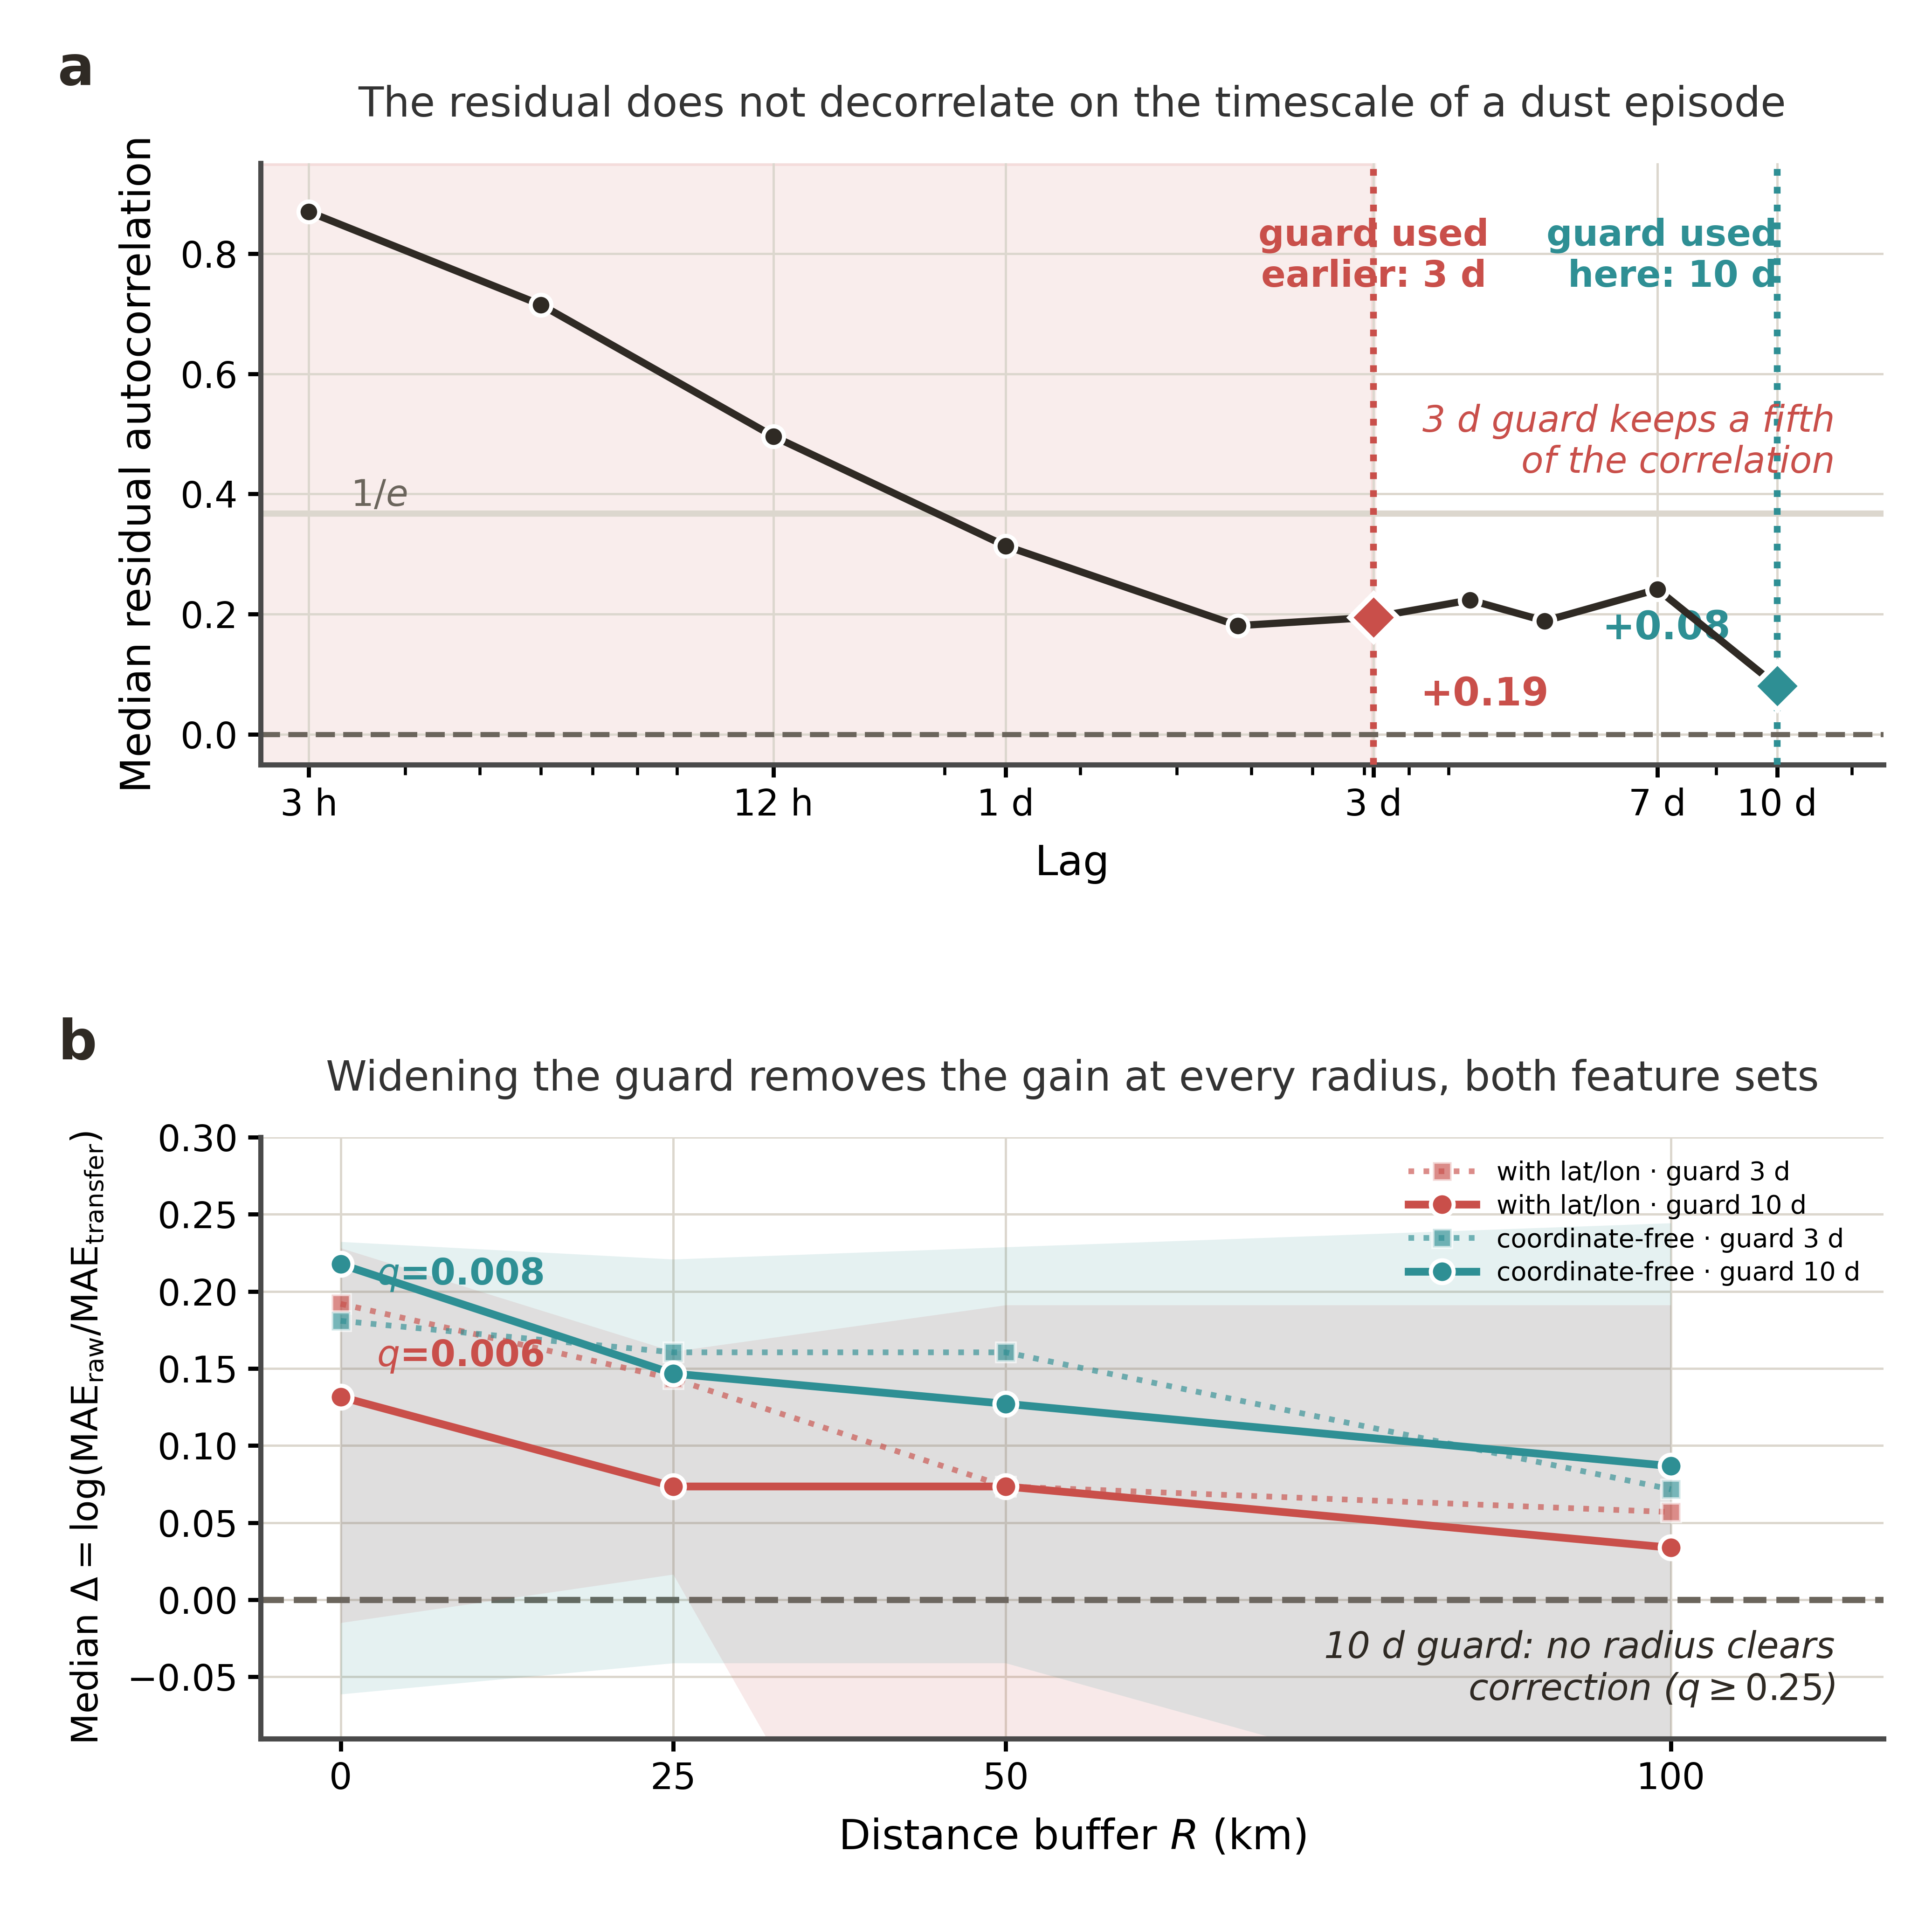
\includegraphics[width=\textwidth]{figures/Empirical_Guard.png}
\caption{The two measured quantities that set the temporal guard.
(a)~Median station-level autocorrelation of the observation-minus-CAMS residual by lag. The
residual is still $+0.19$ at three days and reaches $+0.08$ only at ten days, so a guard taken
from the duration of a dust episode leaves a fifth of the correlation inside the training
window. (b)~Median transfer estimand $\Delta=\log(\mathrm{MAE_{raw}/MAE_{transfer}})$ against
buffer radius for both feature sets under the three-day and the ten-day guard; shading is the
grid-cell block bootstrap. Under the measured ten-day guard no radius clears correction after
Benjamini--Hochberg adjustment ($q\ge0.25$).}
\label{fig:guard}
\end{figure}

\begin{figure}[p]
\centering
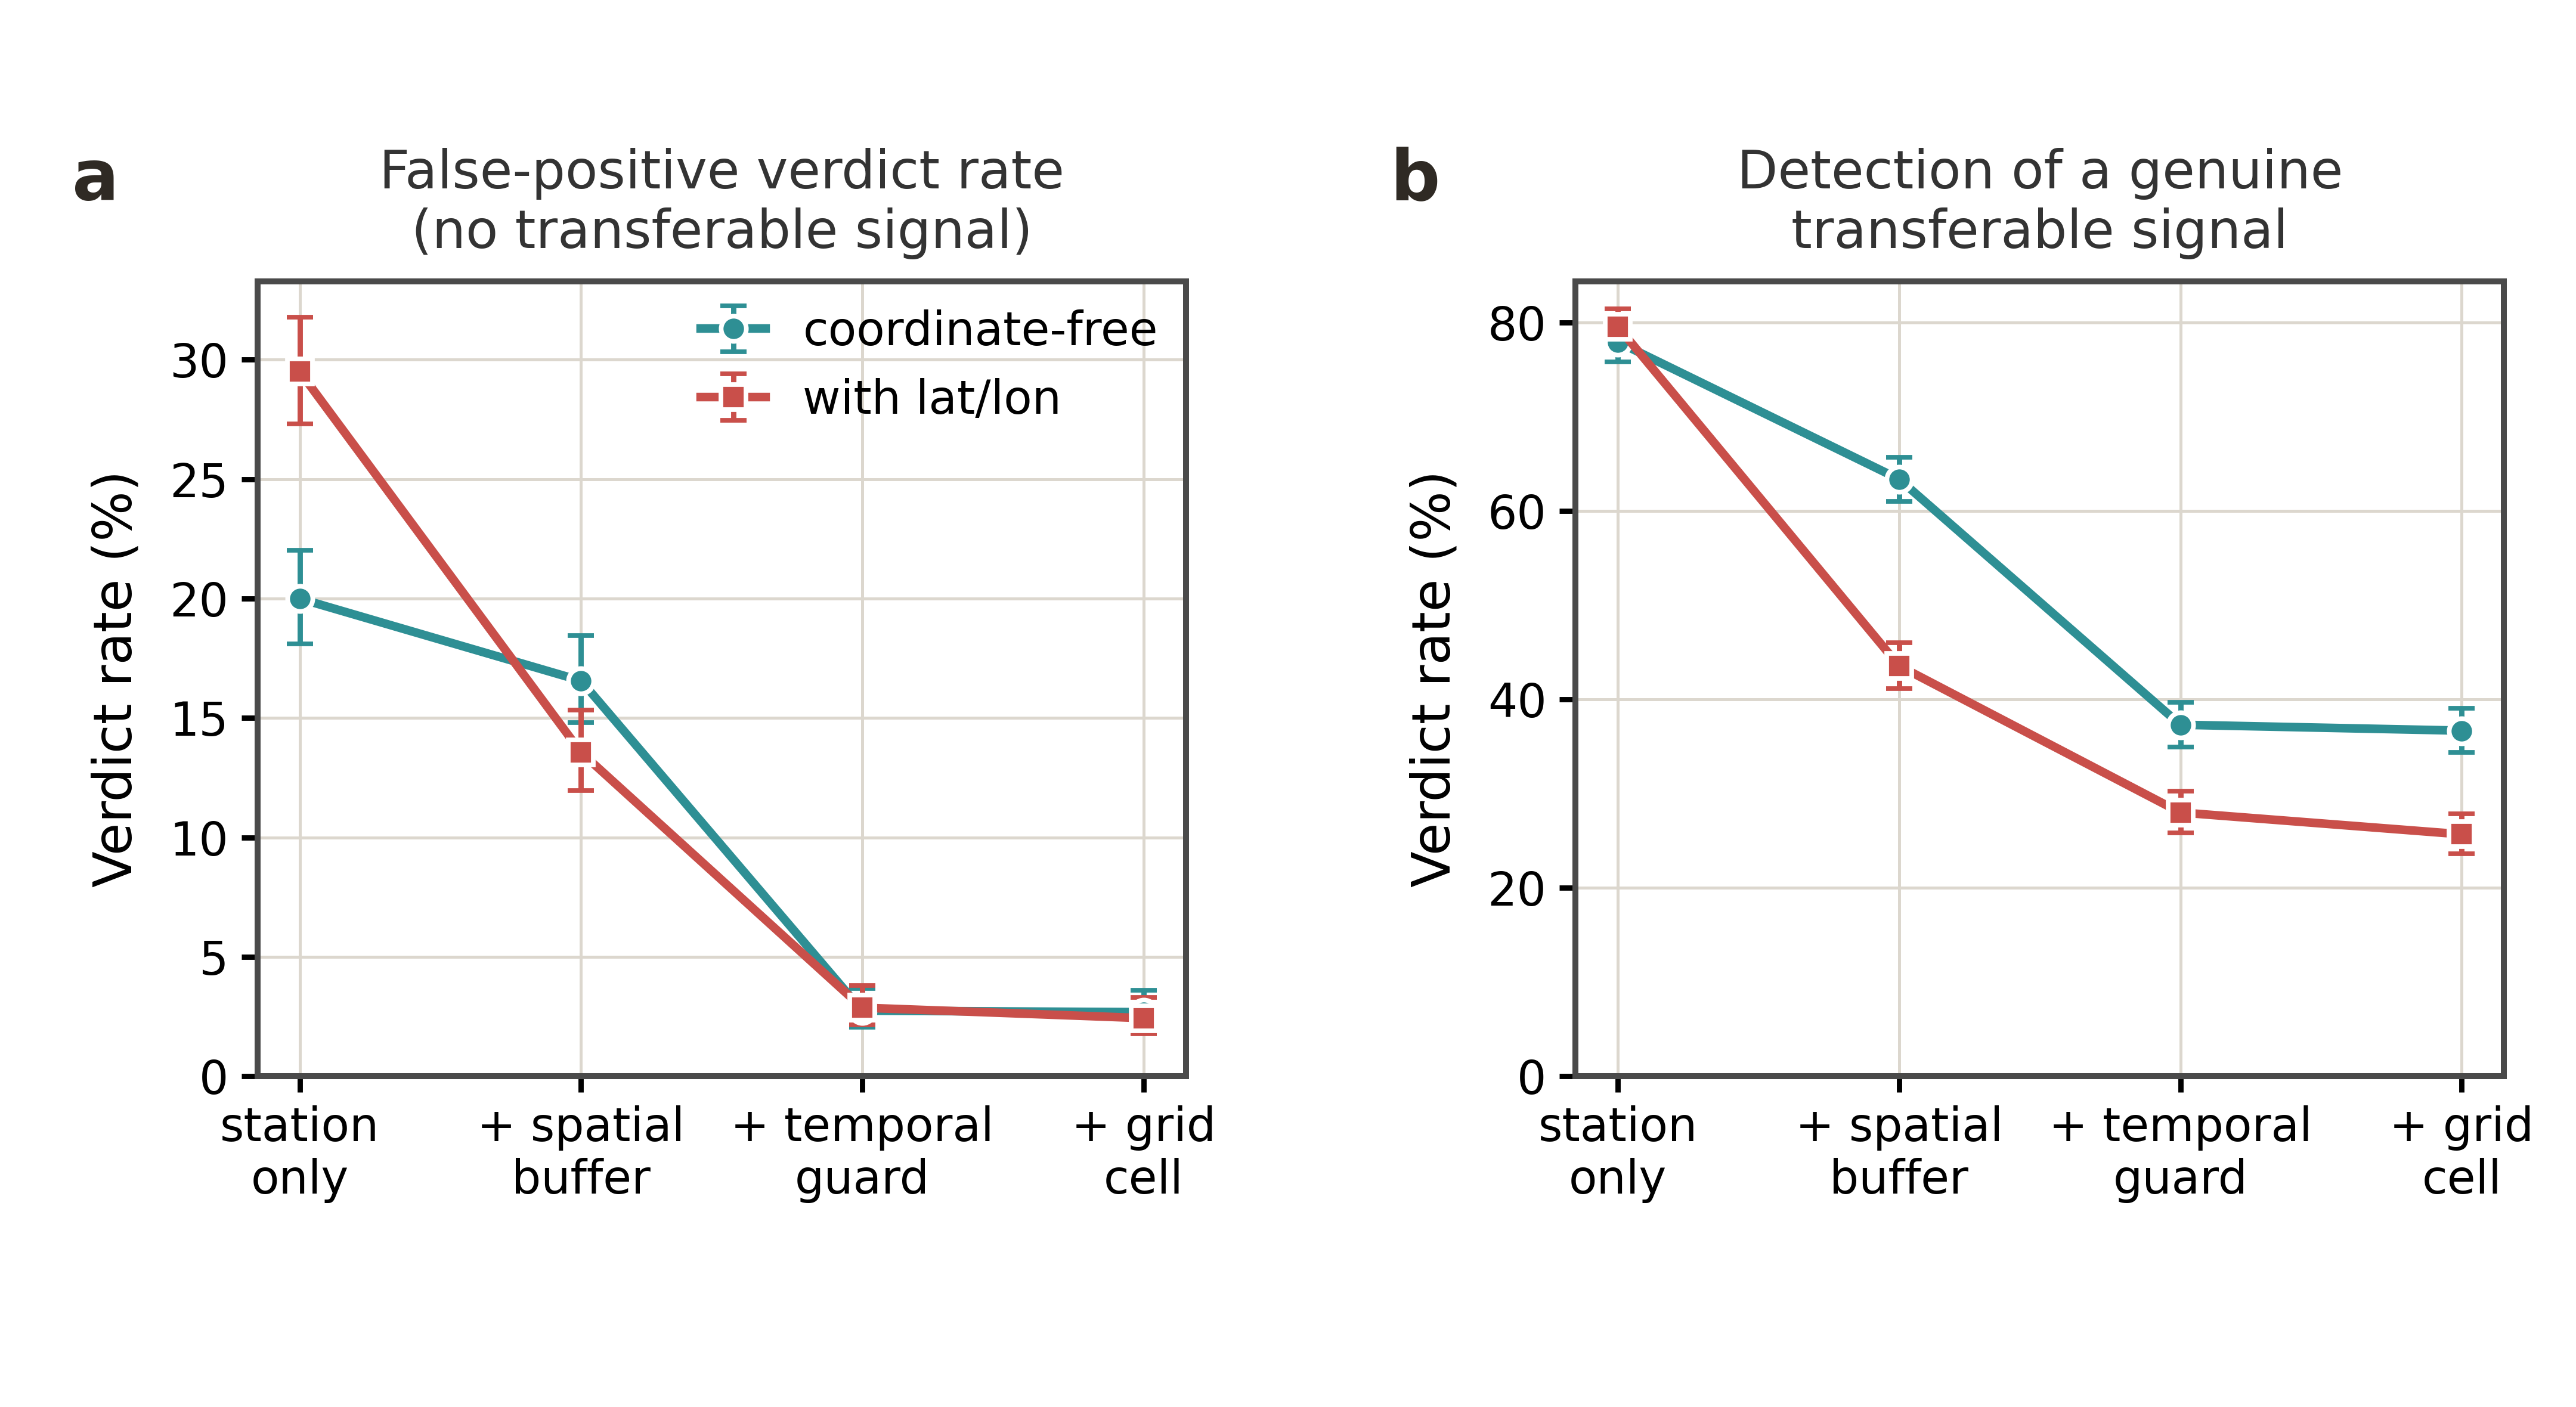
\includegraphics[width=\textwidth]{figures/Simulation_Ladder.png}
\caption{Ground-truth stochastic experiment across the validation ladder, at the primary
$R=50$~km buffer. (a)~False-positive verdict rate when no transferable signal is present.
(b)~Detection of a genuine transferable signal. Bars are Wilson score intervals on the
verdict counts; each point aggregates the pre-declared 32-scenario factorial experiment over
the dependence combinations and the two network geometries. Progressive spatial and temporal
separation sharply reduces false transfer but also reduces detection.}
\label{fig:simladder}
\end{figure}

\begin{figure}[p]
\centering
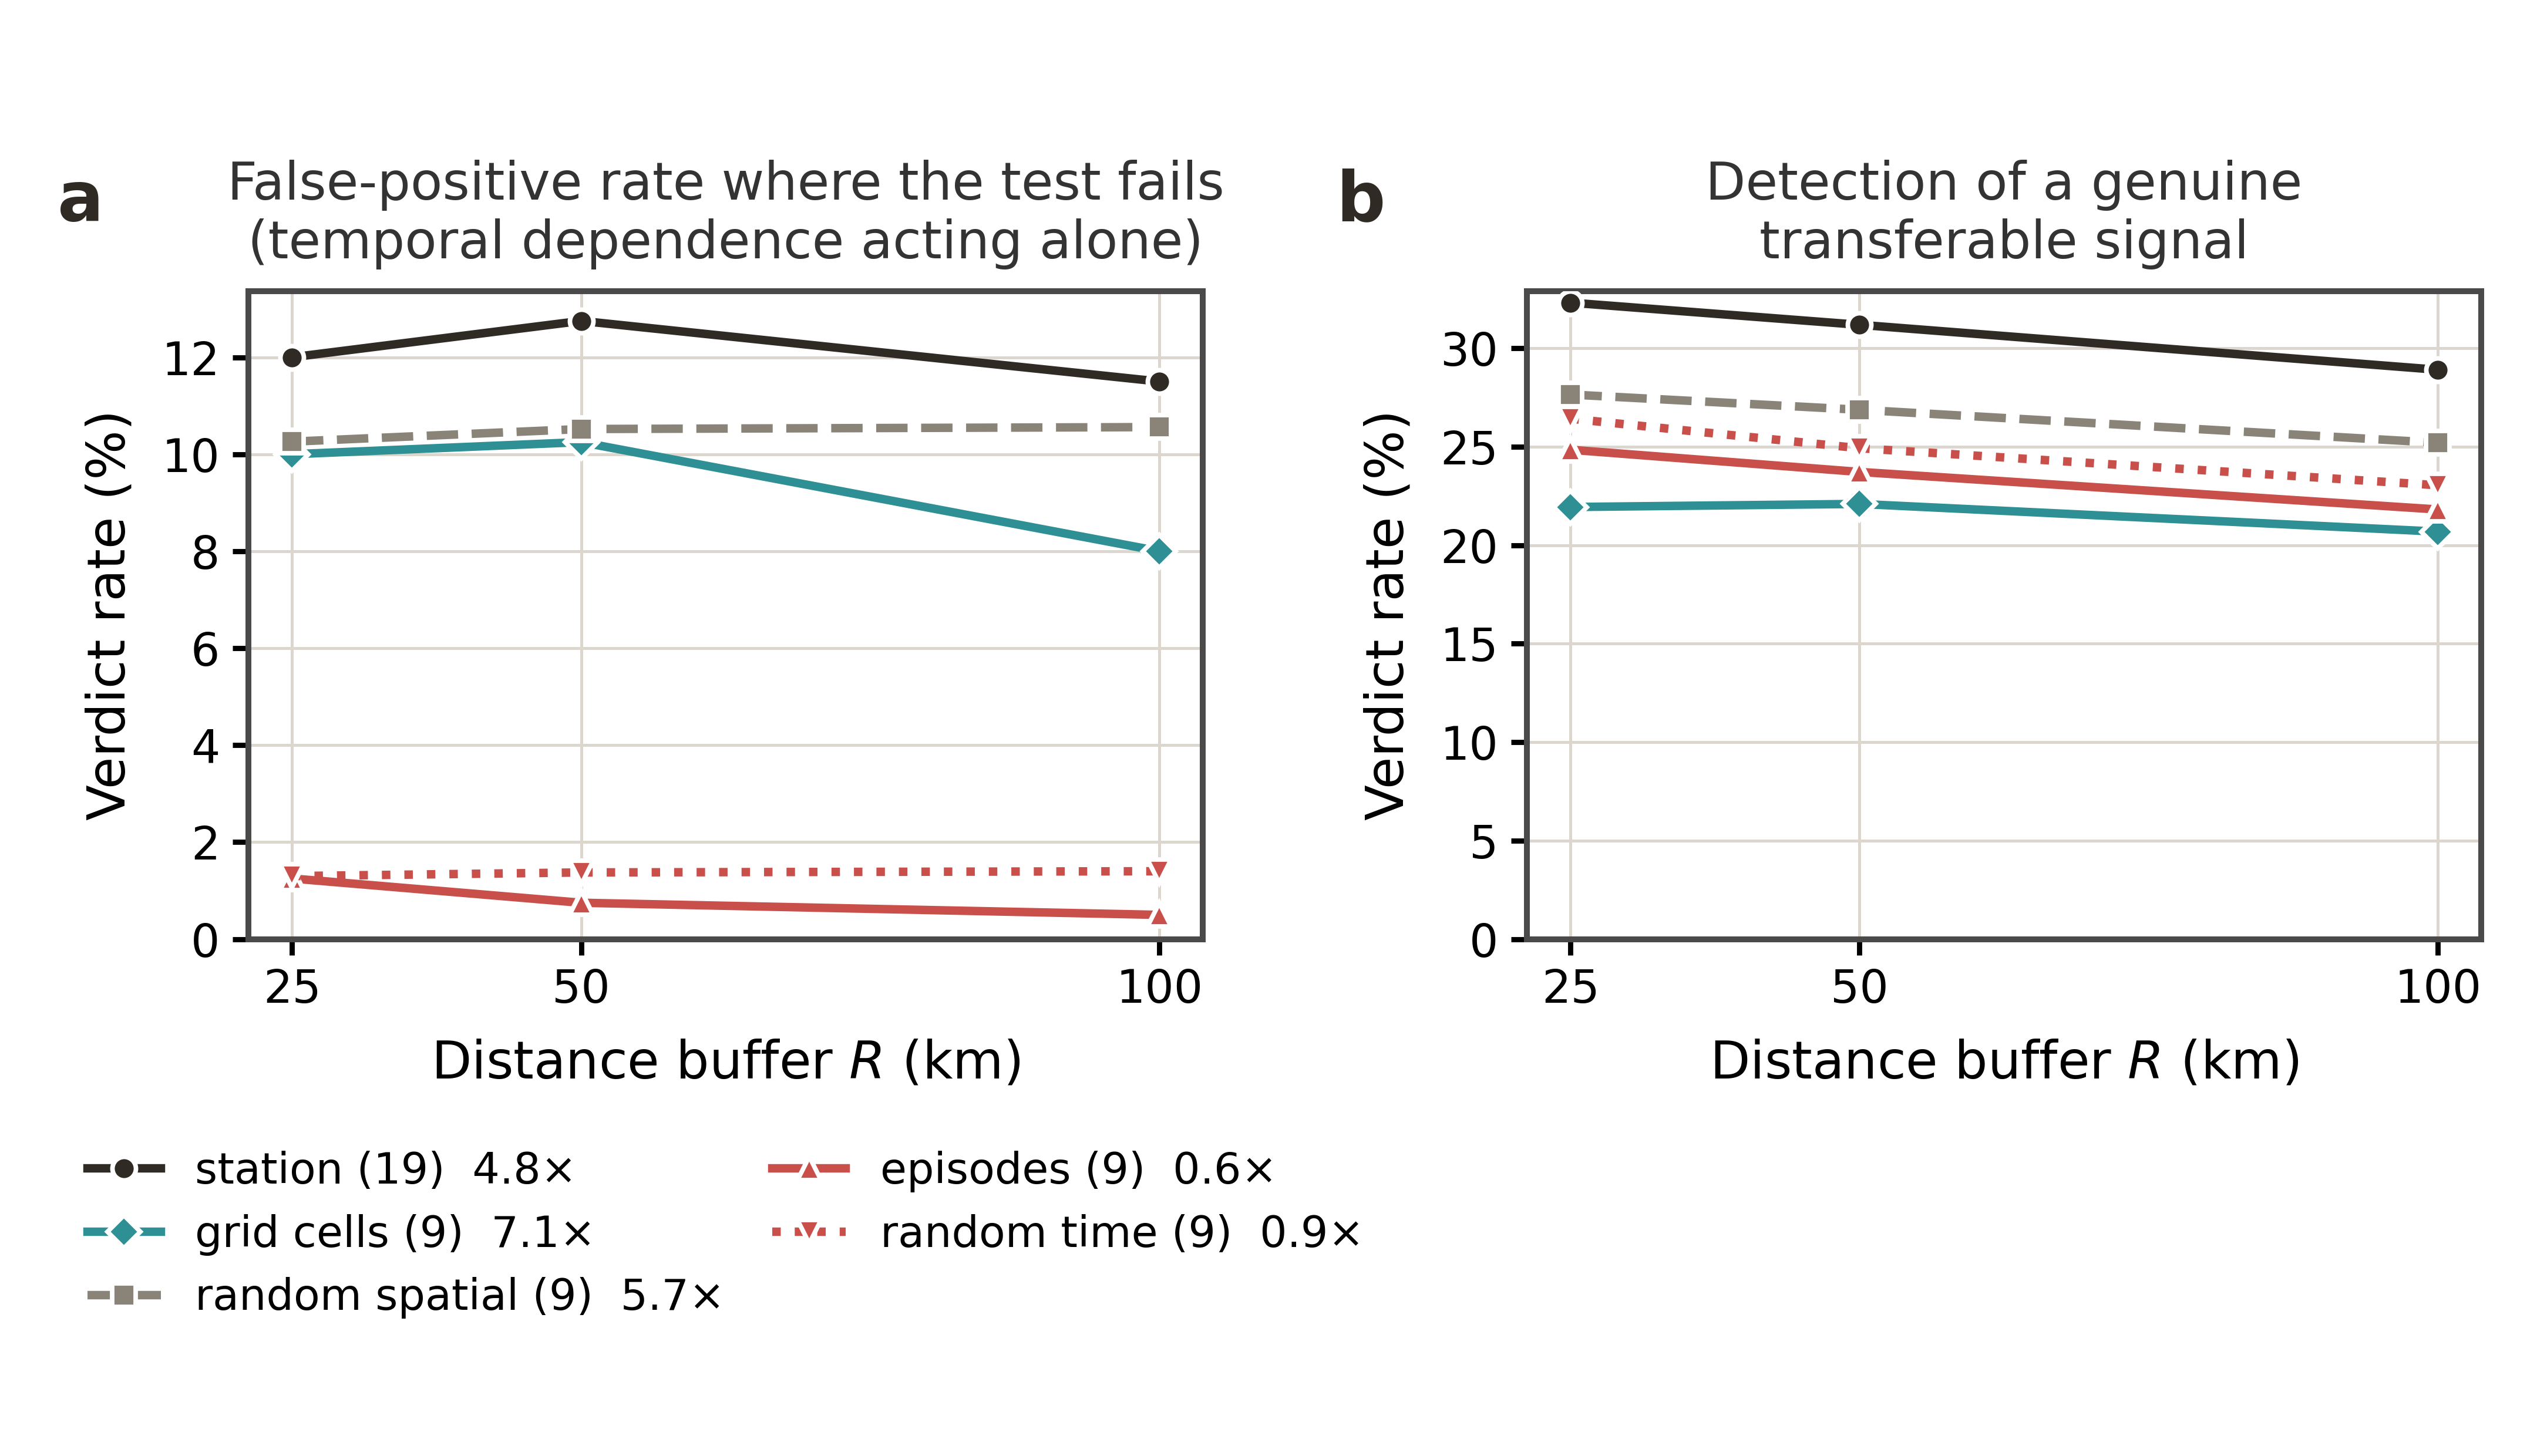
\includegraphics[width=\textwidth]{figures/Unit_Control.png}
\caption{Which inference unit removes the failure, and what it costs. The verdict is a one-sided
exact sign test across held-out units; all five rules are applied to the same realizations, so they
are paired. The station rule counts nineteen targets; the geographic rule the nine occupied
mechanistic-grid cells; the contiguous-episode rule cuts the evaluation window into nine
consecutive blocks; and the two random rules hold the count at nine while destroying the structure
the corresponding structured rule claims to use, averaged over fifty partitions per realization.
(a)~False-positive verdict rate in the corner where the station-level test is anti-conservative:
a residual component common to the network in time, with neither spatial proximity nor shared grid
support. The figure beside each label is that rule's corner rate divided by its own pooled
false-positive rate, which distinguishes a rule that is calibrated here from one that merely
declares transfer less often everywhere; the spatial rules sit between $4.8$ and $7.1$, the
temporal rules at $0.6$ and $0.9$. (b)~Detection of a genuine transferable signal, pooled over the
sixteen scenarios in which one is present. The episode rule costs less detection than the
geographic unit at every radius.}
\label{fig:unitcontrol}
\end{figure}

\end{document}
